\documentclass{beamer}
\usepackage{listings}
\usepackage{minted}
\usepackage{anyfontsize}
\usepackage[utf8]{inputenc}

\mode<presentation> {
  \usetheme{Madrid}
}

\title[Zinc R53 Policy Records for Cheapskates]{Zinc Route53 Policy Records for Cheapskates} % The short title appears at the bottom of every slide, the full title is only on the title page

\author{Radu Ciorba \href{mailto:radu@presslabs.com}{\{radu@presslabs.com\}}} % Your name
\date{\today} % Date, can be changed to a custom date

\begin{document}

\begin{frame}
  \titlepage % Print the title page as the first slide
\end{frame}

\begin{frame}
  \frametitle{whoami}
  \begin{itemize}
  \item Software Developer + Ops @ Presslabs, in Timișoara, Romania
  \item Using Python since 2006
  \item Using Python profesionally since 2010
  \end{itemize}
\end{frame}


\begin{frame}
  \frametitle{Our Problem}
  \begin{itemize}
  \item We run our own CDN
  \item Ideally we want DNS to take a person to the closest set of Edge Nodes
  \item Split requests between nodes in one set, based on weight
  \item Never take them to an unhealthy node
  \end{itemize}
\end{frame}

\begin{frame}
  \frametitle{Solution}
  \begin{itemize}
  \item Use Route 53 Policy Records
  \item 50 EUR * 3 (www, cdn, @) * several hundred customers
  \item Or make www, cdn, @ CNAMEs to cdn.presslabs.com (but that means extra latency)
  \end{itemize}
\end{frame}

\begin{frame}
  \frametitle{Solution 2}
  Policy is made up of Alias records, you can build your own
  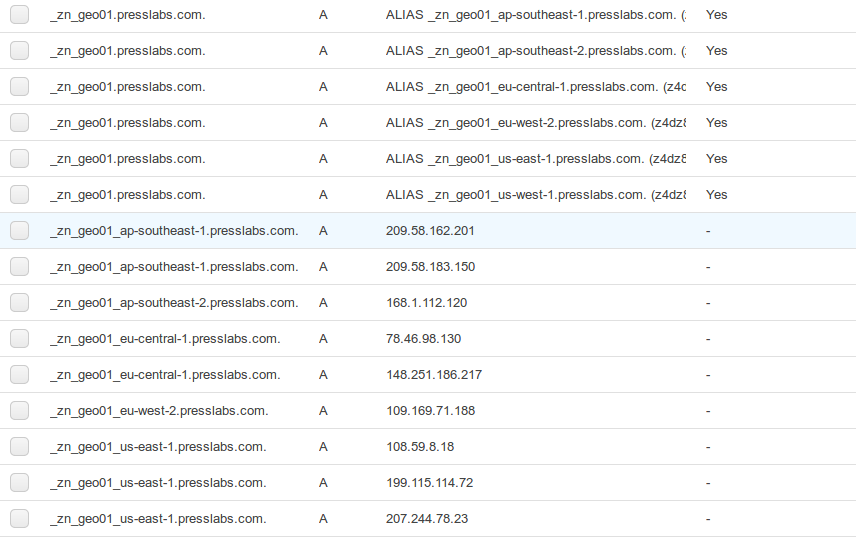
\includegraphics[scale=0.38,keepaspectratio=true]{./images/aws-policy-tree.png}

\end{frame}

\begin{frame}
  \frametitle{So we did. Introducting: Zinc}
  \begin{itemize}
  \item Open Source
  \item Python3
  \item Simple REST API
  \item Good testing, 82\% coverage
  \end{itemize}
\end{frame}

\begin{frame}
  \frametitle{Quick Demo}
  Demo time!
\end{frame}

\begin{frame}
  \frametitle{Thanks}
  You can find the code here:
  \newline
  \href{https://github.com/presslabs/zinc}{https://github.com/presslabs/zinc}
  \newline
  \newline
  If you need hosting for a Wordpress site:
  \newline
  \href{https://presslabs.com}{https://presslabs.com}
\end{frame}
\end{document}
